\documentclass[11pt, a4paper]{article}
\usepackage{polski}
\usepackage[UTF8]{inputenc}
\usepackage{amsmath}
\usepackage{longtable}
\usepackage[pdftex]{graphicx}
\usepackage{wrapfig}
\usepackage{subfig}
\usepackage{sidecap}
\usepackage{makeidx}
\usepackage{enumerate}

\makeindex

\usepackage[bookmarksnumbered,colorlinks,plainpages,backref]{hyperref}
\hypersetup{
 citecolor=[rgb]{0, 0.6, 0},
 linkcolor=[rgb]{0,0.4,0},
 urlcolor=blue}


\author{K.~Narożnik}
\title{Słów kilka\\ O klubie o którym słyszy się na codzień \\
Słów subiektywnych, a jakże\\ Na to co sie dzieje\\ I na to co się dziać będzie\\
W FC BARCELONIE}
\date{08.12.2014}
\linespread{1.4}

\linespread{1.2}
\newcommand{\kwle}{To jest artykuł o Barcelonie}
\begin{document}
\maketitle

\newpage
\tableofcontents
\newpage

\section{Ogólnie o Barcelonie}
\label{sec:Ogolnie}

Futbol Club Barcelona (w języku katalońskim), w skrócie Barca – kataloński wielosekcyjny klub sportowy, istniejący od chwili założenia drużyny piłkarskiej. Założony w 1899 przez grupę Szwajcarów, Anglików i Hiszpanów, z czasem stał się katalońską instytucją o dużym znaczeniu społecznym. Jedna z wielu teorii mówi, że barwy klubowe Barcelona zaczerpnęła od szwajcarskiego klubu FC Basel.

Drużyna piłkarska należy do najbardziej utytułowanych zespołów świata w tej dyscyplinie – ma na koncie dwadzieścia dwa mistrzostwa Hiszpanii, dwadzieścia sześć Pucharów Króla Hiszpanii, dziesięć Superpucharów Hiszpanii, cztery Puchary Europy, cztery Puchary Zdobywców Pucharów, cztery Superpuchary Europy, dwa razy Klubowe Mistrzostwo Świata/Puchar Interkontynentalny i wiele innych trofeów.

Klub ma 162 979 socios – członków klubu – i miliony culés na całym świecie, z których część zrzeszona jest w penyach, czyli oficjalnych fanklubach, których jest 1054. Posiada również rozbudowaną infrastrukturę – stadiony Camp Nou, Mini Estadi, miasteczko sportowe Ciutat Esportiva Joan Gamper, szkółkę La Masía i halę Palau Blaugrana, w której rozgrywają swoje mecze zawodnicy innych sekcji.

Poza sekcją piłkarską do FC Barcelona należą jeszcze: Regal FC Barcelona, FC Barcelona-Intersport, FC Barcelona Sorli Discau i FC Barcelona Senseit). Klub posiada także rezerwową i młodzieżową drużynę piłki nożnej (FC Barcelona B), a także liczne sekcje amatorskie.

Drużyna z Camp Nou na arenie międzynarodowej startuje nieprzerwanie od 50 lat, czyli od początku powstania europejskich pucharów. Jest jednym z trzech klubów, które od założenia Primera División, czyli od 1929 roku, nieprzerwanie grają w najwyższej klasie rozgrywkowej Hiszpanii.

Drużyna z Camp Nou na arenie międzynarodowej startuje nieprzerwanie od 50 lat, czyli od początku powstania europejskich pucharów. Jest jednym z trzech klubów, które od założenia Primera División, czyli od 1929 roku, nieprzerwanie grają w najwyższej klasie rozgrywkowej Hiszpanii.

\section{Matma w Barcelonie}
\label{sec:Matma}
Cóż, Barca ma też stały wzór na liczbę punktów pod koniec sezonu. Jest on taki:
$$\frac{liczba~symulek~Neymara\index{Neymar}}{bramki~CR7} * {ugryzienia~Suareza\index{Suarez}}$$
Można też policzyć to inaczej, bo układem równań z innymi zmiennymi, gdzie y to miejsce pod koniec sezonu :
\begin{equation}
	y = \left\{	
	\begin{array}{ll}
	odbiory~Busquetsa\index{Busquets} & \textrm{jeżeli $odbiory > 0 \land CR7 <0$} \\
	sprinty~Pique\index{Pique} & \textrm{jeżeli $sprinty > 0 $} \\
	1 & \textrm{gdy Messi\index{Messi} strzeli więcj niż 40 goli}
		
	\end{array} \right.
	\label{eq:nr1}
\end{equation}
\section{Piłkarze Barcelony}
\label{sec:Pilkarze}
\begin{longtable}{|l|l|r|r|r|}
\caption{Piłkarze Barcelony}\\\hline
\multicolumn{5}{|c|}{Wybrani piłkarze sezonu 2014/15}\\\hline
imie & nazwisko & pozycja & mecze & gole \\ \hline
\endfirsthead
\hline
\multicolumn{5}{|c|}{Wybrani piłkarze sezonu 2014/15}\\
imie & nazwisko & pozycja & mecze & gole \\ \hline
\endhead
\hline \multicolumn{5}{|c|}{Wybrani piłkarze sezonu 2014/15}\\ \hline
\endfoot
\hline \multicolumn{5}{|c|}{Wybrani piłkarze sezonu 2014/15}\\
\hline
\endlastfoot
Claudio & Bravo\index{Bravo} & BR & 13 & 0 \\
Dani  & Alves \index{Dani Alves} & PO & 11 & 0 \\
Marc & Bartra \index{Bartra} & ŚO & 5 & 0 \\
Gerard & Pique \index{Pique} & ŚO & 9 & 1 \\
Javier  & Mascherano & ŚO & 9 & 0 \\
Jordi & Alba & LO & 13 & 1 \\
Andres & Iniesta & ŚPO & 13 & 3 \\
Xavier  & Hernandes & ŚP & 5 & 0 \\
Sergio & Busquets & ŚPD & 11 & 1 \\
Neymar & & LS & 13 & 11 \\
Lionel  & Messi & NP & 14 & 16 \\
Luiz & Suarez & NP & 8 & 0 \\
Ivan & Rakitić & ŚP & 6 & 2 \\
Jeremy & Mathieu & ŚO & 6 & 1 \\
Pedro &  & PS & 8 & 2 \\
Adriano &  & LO & 3 & 0 \\
\end{longtable}
\section{Najnowsze informacje o Barcelonie}
\subsection{Nowy trener - Luiz Enrique}
\begin{wrapfigure}{r}{0.5\textwidth}
\begin{center}
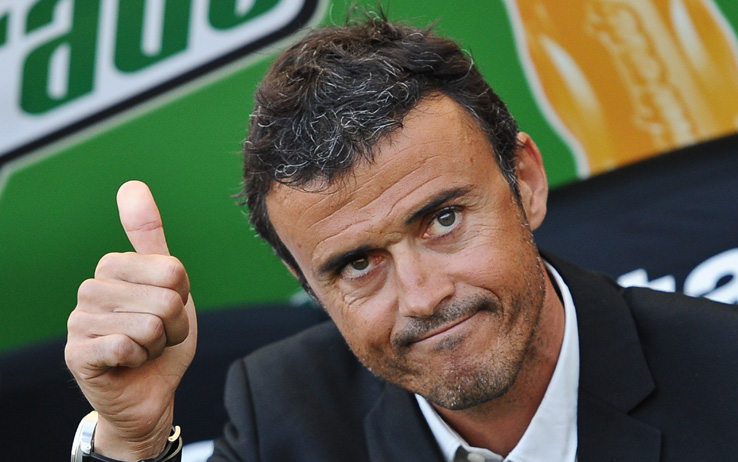
\includegraphics[width=0.48\textwidth]{luzienrique.jpg}
\end{center}
\caption{Luiz Enrique\cite{Enrique}}
\label{img:Luiz}
\end{wrapfigure}
\index{Luiz Enrique}
Najnowsza historia Barcy optymistyczna nie jest. Trenerem od nowego sezonu został Luiz Enrique.
16 maja 2014 roku Enrique ogłosił, że opuszcza Celtę Vigo. Dwa dni później podpisał dwuletni kontrakt z Barceloną. Jednak drużyna nie gra, tak, jakby oczekiwali kibice i coraz więcej jest głosów ay podziękowac za współpracę wychowankowi Barcelony.

Mówiliśmy o Celcie Vigo. Tam, Enrique spisywał się nadzwyczajnie dobrze. Razem z innym wychowankiem Barcelony - Rafinhą \index{Rafinha}, który grał w Celcie na pozycji pomocnika, udało sie uzyskać wysokie, dziewiąte miejsce w Primiera Division.

\begin{wrapfigure}{l}{0.5\textwidth}
\begin{center}
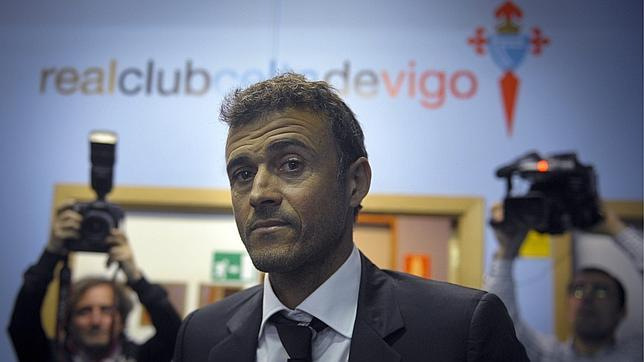
\includegraphics[width=0.48\textwidth]{enrique2.jpg}
\end{center}
\label{img:Luiz2}
\end{wrapfigure}
\index{Luiz Enrique}
Drużyna Hiszpana grała stylem określanym "stylem Barcelony" polegającym na dużej ilości podań, zakładaniu szybkiego i skutecznego pressingu oraz na częstej wymianie pozycji. W Vigo to działało, a wszyscy byli zachwyceni grą drużyny wychowanka Barcelony. Wydawało się że to idealny trener, aby przejąć zespół po Gerardo Martino.

Jednak wystarczy przyjrzeć się dokładniej karierze trenerskiej Enrique aby zobaczyć, że różowo nie było zawsze. Przed pracą w Celcie był trenerem AS Romy, gdzie zaliczył najgorszy okres w histori rzymskiego klubu. Zwolniono go po dwóch sezonach, w których nie wygrał nic, co więcej nie zakwalifikował się nawet do Ligi Mistrzów.
\newpage

\subsection{Transfery}
\begin{wrapfigure}{l}{0.5\textwidth}
\begin{center}
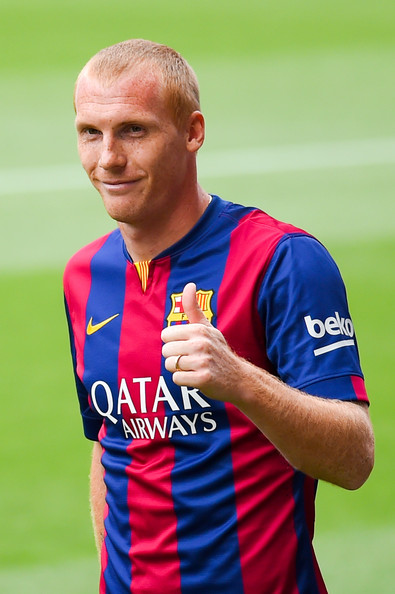
\includegraphics[width=0.42\textwidth]{mathieu.jpg}
\end{center}

\label{img:Mathieu}
\end{wrapfigure}
Jeremy Mathieu \index{Mathieu}23 lipca 2014 roku przeszedł z Valencii do FC Barcelony. Francuz kosztował Dumę Katalonii 20mln euro \footnote{4 miliony zapłacił co ciekawe sam.}. Od początku zadziwiono się ceną Francuza. W Valencii spisywał się ok, jednak wątpiono aby 30-latek warty był tyle pieniedzy. Występuje często w środku obrony czy na lewej stronie zmieniajac Jordiego Albę \index{Alba}, jednak zdania są podzielone. Niektórzy twierdzą, że gra rewelacyjnie, niektórzy że gra kompletnie beznadziejnie i rtuje go tylko bramkarz i reszta obrony. Jednak to że zdania są podzielone utrzymuje że Mathieu aż tak rewelacyjny nie jest. Drugim kupionym obrońcą jest Belg Vermalen\index{Vermalen}. On jednak wciąż leczy kontuzje a kosztował... tyle co Mathieu.

\begin{wrapfigure}{r}{0.48\textwidth}
\begin{center}
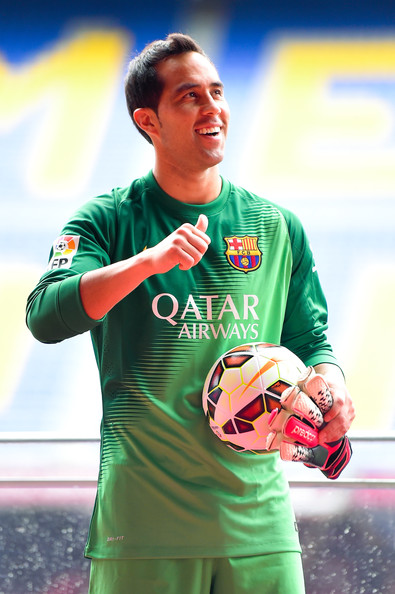
\includegraphics[width=0.24\textwidth]{bravo.jpg}
\end{center}
\label{img:Bravo}
\end{wrapfigure}
Bramkarze ratują sytuację Barcelony, w przeciwieństwie do obrońców. Na początku sezonu kupiono Ter-Stegena, ponieważ Victor Valdes postanowił odejść z klubu. Wydawało się że to on będzie podstawowym bramkarzem, ale wtedy kupiono... 30-letniego Claudio Bravo\index{Bravo}\cite{Bravo} z Realu Sociedad San Sebastian. Okazało się to strzałem w dziesiątkę i Bravo\index{Bravo} jest najlepszym bramkarzem ligi.
\newpage


Do Barcelony przyszło w okienku letnim wielu zawodników. Urugwajczyk i najlepszy strzelec Liverpoolu Luiz Suarez, Chorwat Ivan Rakitić, zdobywca Pucharu UEFA, a także Ter Stegen, najbardziej perspektywiczny młody bramkarz w Europie.

\begin{figure}
\centering
\subfloat[Suarez]{\label{suarez}
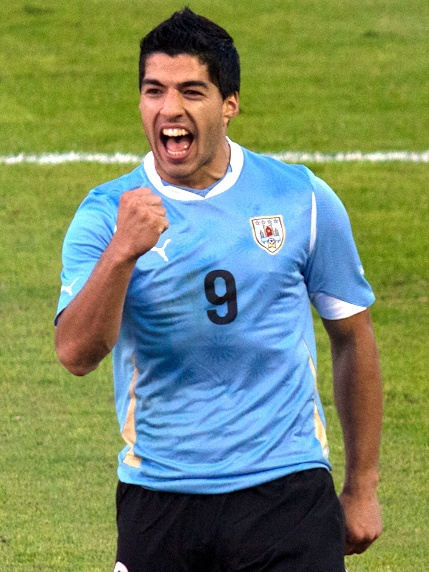
\includegraphics[width=0.4\textwidth]{suarez.jpg}}
\quad
\subfloat[Rakitić]{\label{rakitic}
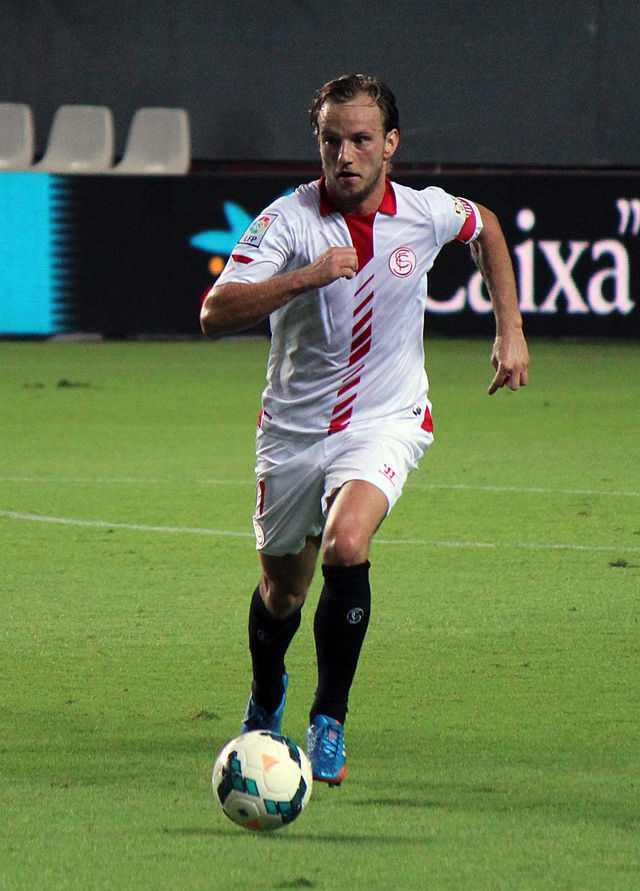
\includegraphics[width=0.4\textwidth]{rakitic.jpg}}
\quad
\subfloat[Ter Stegen]{\label{terstegen}
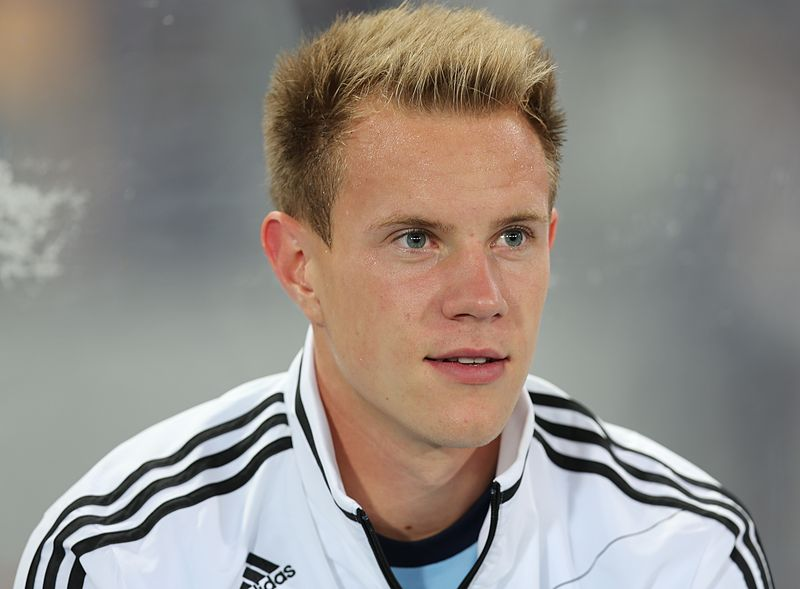
\includegraphics[width=0.4\textwidth]{terstegen.jpg}}
\caption{Nowi w Barcelonie}
\label{fig:animals}
\end{figure}

Na koniec podsumuję to kontrowersyjną wypowiedzią Zubizarety, aby podkreślić swój subiektywizm.
\begin{quote}
(...)Tello jest nawet lepszy niż Cristiano, dla mnie każdy piłkarz FC Barcelona jest od niego lepszy.
\end{quote}
\newpage

\section{Inne, nie wiem gdzie indziej wstawić}
\begin{figure}[!ht]
\centering
\setlength{\unitlength}{0.75mm}
\begin{picture}(60,40)
\put(20,20){\vector(2,0){30}}
\put(10,20){\vector(2,1){25}}
\put(30,20){\vector(3,1){10}}
\put(40,20){\vector(3,1){10}}
\put(25,20){\vector(1,2){15}}
\thicklines
\put(15,20){\vector(-4,1){16}}
\put(19,20){\vector(-1,4){5}}
\thinlines
\put(30,20){\vector(-1,-4){5}}
\end{picture}
\caption{Coścoś}
\label{fig:strzaleczki}
\end{figure}

Przykład new commanda:\\
\kwle;

\newpage
\begin{thebibliography}{9}
\bibitem{Enrique} Wikipedia : \emph{http://pl.wikipedia.org/wiki/Luis\_Enrique}

\bibitem{Bravo}  Wikipedia : \emph{http://pl.wikipedia.org/wiki/Claudio\_Bravo}


\end{thebibliography}
\printindex
\end{document} 